
%!TEX TS-program = xelatex
%!TEX encoding = UTF-8 UnicodeWhat is at-issueness? An experimental comparison of diagnostics

\documentclass[compress, xcolor = dvipsnames, aspectratio=169]{beamer}

%fonts
	\usepackage{fontspec}
	\setmainfont[Scale=MatchLowercase,Mapping=tex-text]{Linux Biolinum}
	\setsansfont[Scale=MatchLowercase,Mapping=tex-text, BoldItalicFeatures={FakeBold=3}]{Linux Biolinum}
	\newfontfamily\opt{Optima}
	\usepackage{pifont}% http://ctan.org/pkg/pifont
	\newcommand{\cmark}{\ding{51}}%
	\newcommand{\xmark}{\ding{55}}%

%metadata
	\title{{\bfseries What is at-issueness? An experimental comparison of diagnostics}}
	\author{Conglei Xu, Lisa Hofmann, Judith Tonhauser\\[.5\baselineskip]
		\scriptsize lisa.hofmann@ling.uni-stuttgart.de}
	\institute{
\includegraphics[width=.3\textwidth]{../uni-logo-b.png}}
	\date{\small Experiments on the semantics/pragmatics interface (XPrag fest 2025)\\
	    	July 18st, 2025}

%theme
	\usetheme{default}
	\setbeamertemplate{navigation symbols}{}
	\setbeamertemplate{headline}{
		\begin{beamercolorbox}{section in head/foot}
			\opt\vskip3pt\insertnavigation{\paperwidth}
		\end{beamercolorbox}
	}
	\setbeamertemplate{footline}[frame number]

	\setbeamerfont{title}{family = \opt, series = \bfseries}
	\setbeamerfont{frametitle}{family = \opt, series = \bfseries}
	\setbeamerfont{headline}{family = \opt}

%color scheme
	% screen template
	\definecolor{bgyellow}{HTML}{FFFCF7}
	\definecolor{normaltext}{HTML}{505050}
	\definecolor{highlights}{HTML}{2a6d8c}

	\setbeamercolor{background canvas}{bg=bgyellow}
	\setbeamercolor{normal text}{fg=normaltext}
	\setbeamercolor{palette primary}{fg=highlights}
    \setbeamercolor{palette secondary}{fg=highlights}
    \setbeamercolor{palette tertiary}{fg=highlights}
    \setbeamercolor{palette quaternary}{fg=highlights}
    \setbeamercolor{structure}{fg=highlights}

    \setbeamertemplate{enumerate items}[circle]

% !TeX root = asymmetries-local-contexts.tex
%layout, formatting
	\usepackage[round]{natbib}
	\usepackage{multicol}
	\usepackage{linguex}
	\usepackage{multirow}
	\usepackage{colortbl}
	\usepackage{booktabs}
	\usepackage{array}
	\usepackage{hyperref}

%text features
	\usepackage{csquotes}
	\usepackage{stmaryrd}
	\usepackage[normalem]{ulem} % sout

%macros
	\newcommand{\listref}[1]{\phantom{.}\hfill {\scriptsize [#1]}}
	\newcommand{\transl}{\ensuremath\rightsquigarrow}

% drawing 
	\usepackage{tikz}
	\usepackage{venndiagram}
	\usepackage{easybmat}

% diagram shortcuts
	\usetikzlibrary{calc}
	\tikzstyle{index gray}=[inner sep=2pt, black, circle, fill=lightgray]
	\tikzstyle{opaque}=[fill=gray,fill opacity=.1]
	\newcommand{\indices}{% Indices
	    \draw (-1,1) node[index gray] (yy) {$w_{us}$};
	    \draw (1,1) node[index gray] (yn) {$w_u\phantom s$};
	    \draw (-1,-1) node[index gray] (ny) {$w_s\phantom u$};
	    \draw (1,-1) node[index gray] (nn) {$w_0\phantom i$};
		}


% propositions
	\newcommand{\sprop}{% s proposition
		\draw[rounded corners] (-1.9,1.9) rectangle (-.1, -1.9);}
	\newcommand{\uprop}{% u proposition
		\draw[rounded corners] (-1.9,1.9) rectangle (1.9,.1);}
	\newcommand{\nsprop}{% ~s proposition
		\draw[rounded corners] (1.9,-1.9) rectangle (.1, 1.9);}

% contexts
	\newcommand{\ccontext}{% c context
		\draw[opaque, rounded corners] (-1.8,1.8) rectangle (1.8, -1.8);}

	\newcommand{\ucontext}{% u context
		\draw[opaque, rounded corners] (-1.8,1.8) rectangle (1.8,.2);}
	\newcommand{\nucontext}{% ~u context
		\draw[opaque, rounded corners] (-1.8,-1.8) rectangle (1.8,-.2);}
	\newcommand{\scontext}{% s context
		\draw[opaque, rounded corners] (-1.8,1.8) rectangle (-.2, -1.8);}
	\newcommand{\nscontext}{% ~s context
		\draw[opaque, rounded corners] (1.8,1.8) rectangle (.2, -1.8);}
	
	\newcommand{\unscontext}{% u + ~s context
		\draw[opaque, rounded corners] (.2,1.8) rectangle (1.8,.2);}
	\newcommand{\uscontext}{% u + s context
		\draw[opaque, rounded corners] (-.2,1.8) rectangle (-1.8,.2);}
	\newcommand{\nuscontext}{% ~u + s context
		\draw[opaque, rounded corners] (-.2,-1.8) rectangle (-1.8,-.2);}
	\newcommand{\zerocontext}{% u + ~s context
		\draw[opaque, rounded corners] (.2,-1.8) rectangle (1.8,-.2);}

	\newcommand{\undefined}{% undefined context
		\draw[thick, Magenta] (-1.9,1.9) -- (1.9,-1.9);
		\draw[thick, Magenta] (-1.9,-1.9) -- (1.9,1.9);}
	
	\newcommand{\negquitwoqud}{% c context
		\draw[opaque, rounded corners] (-1.8,1) -- (-1.8,1.8) -- (.1,1.8) -- (.1,.1) -- (1.8,.1) -- (1.8, -1.8) -- (-.1, -1.8) -- (-.1, -.1) -- (-1.8, -.1) -- (-1.8,1);}
	\newcommand{\nquitcontext}{% not quit context
		\draw[opaque, rounded corners] (-1.8,0) -- (-1.8,1.8) -- (-.2,1.8) -- (-.2,-.2) -- (.2,-.2) -- (1.8,-.2) -- (1.8, -1.8) -- (-1.8, -1.8) -- 
		(-1.8,0);}

% local contexts
	\newcommand{\uslocal}{% u+s local context
		\draw[rounded corners] (-1.8,1.8) rectangle (-.2,.2);}
	\newcommand{\unslocal}{% u+~ns local context
		\draw[rounded corners] (1.8,1.8) rectangle (.2,.2);}
	\newcommand{\unslocalnudge}{% u+~ns local context
		\draw[rounded corners, xshift=-.1cm,yshift=-.1cm ] (1.8,1.8) rectangle (.2,.2);}
	

% input contexts
	\newcommand{\cinput}{% c input context
		\draw[dashed, rounded corners] (-1.9,1.9) rectangle (1.9, -1.9);}
	\newcommand{\uinput}{% u input context
		\draw[dashed, rounded corners] (-1.9,1.9) rectangle (1.9,.1);}
	\newcommand{\nuinput}{% u input context
		\draw[dashed, rounded corners] (-1.9,-1.9) rectangle (1.9,-.1);}
	\newcommand{\sinput}{% s input context
		\draw[dashed, rounded corners] (-1.9,1.9) rectangle (-.1, -1.9);}
	\newcommand{\nsinput}{% ~s input context
		\draw[dashed, rounded corners] (1.9,-1.9) rectangle (.1, 1.9);}


	% distance graph
	\newcommand{\distancegraph}{
    	\draw[->] (yn) -- (yy);   % yy → yn
    	\draw[->] (yn) -- (nn);   % yn → nn
	    \draw[->] (yy) -- (ny);   % yy → ny
	    \draw[->] (nn) -- (ny);   % ny → nn
        \draw (yn) circle (0.33);         % inner circle (node border is ~0.25 cm)
	    \draw (yn) circle (0.39);
		}
	\newcommand{\classes}{	
		\draw[shorten <= -1cm, shorten >= -1cm] ($(yy)!0.5!(yn)$) -- ($(yn)!0.5!(nn)$);
		\draw[shorten <= -1cm, shorten >= -1cm] ($(yy)!0.5!(ny)$) -- ($(ny)!0.5!(nn)$);}
	\newcommand{\classlabels}{
		\node at ($(yn)+(0.8,0.5)$) {$d=0$};                 % region containing w_u
		\node at ($(yy)!0.5!(nn)$)   {$d=1$};                 % region containing w_{us}, w_0
		\node at ($(ny)+(-0.8,-0.5)$){$d=2$}; 
	}




\begin{document}

\begin{frame}
\titlepage

\end{frame}

\section{Introduction}
	\begin{frame}\frametitle{At-issueness}\small

		% Central concept in semantics \& pragmatics:\\ 
		Distinguish propositional content expressing the main point of an utterance (at-issue content) from those conveying background information (not-at-issue content) \pause

		\ex. \emph{Greg, who bought a new car, is envied by his neighbor.}
			\a. At-issue content: \emph{Greg is envied by his neighbor}
			\b. Not-at-issue content: \emph{Greg bought a new car}\pause
			\z.\z.
		
		\begin{itemize}
			\item Several definitions and diagnostics have been proposed in the literature\pause

			\item Very little discussion of whether definitions and diagnostics target the same underlying phenomenon (\citealt{snider_anaphoric_2017,snider_at-issuenessne_2017,snider_distinguishing_2018,koev_notions_2018,faller_discourse_2019,korotkova_evidential_2020})\pause

			\item This work: take a step in adressing this question, compare whether four commonly used diagnostics yield the same results for propositional contents introduced by the same kinds of expressions

			% \item exp 1--4 overview

		\end{itemize}
	
	\end{frame}

	\begin{frame}\frametitle{Experiments 1–4}
		\begin{itemize}
			\item Across four experiments, we manipulated the diagnostic used to assess the at-issueness status of the same contents\pause

			\item We chose four diagnostics that have been suggested to target different notions of at-issueness and show different empirical patterns (\citealt{snider_anaphoric_2017,snider_at-issuenessne_2017,snider_distinguishing_2018,koev_notions_2018,faller_discourse_2019,korotkova_evidential_2020})\pause

			\item We offer a systematic experimental comparison

		\end{itemize}
			
	\end{frame}

	\begin{frame}[t]\frametitle{Question-based at-issueness diagnostics}\small

		Question-based diagnostics assume a conception of at-issueness relative to the QUD: At-issue content is the part of an utterance that interacts with the current QUD (\citealt{amaral_review_2007,simons_what_2010})\pause

		\ex. \label{qud}%
		    QUD diagnostic (e.g., \citealt{tonhauser_diagnosing_2012,chen_presuppositions_2024})
		    \a.[A:] \emph{What did Greg buy?}
		    \b.[B:] \emph{Greg, who bought a new car, is envied by his neighbor.}
		    \z.
		    Question to participants: How well does B's response fit A's question?\pause
		  \z.
		  %
		  % \vspace{-1.5\baselineskip}

		  %
		  \ex. \label{aw}%
		    `asking whether' diagnostic (e.g., \citealt{tonhauser_how_2018,solstad_cataphoric_2024})\smallskip\\
		      \emph{Is Greg, who bought a new car, envied by his neighbor?}\smallskip
		  \\ Question to participants: Is the speaker asking whether Greg bought a new car?\pause
		  \z.
		  % \vspace{-1.5\baselineskip}


		\begin{itemize}
			% \item Four diagnostics
			\item Other diagnostics make other assumptions
			(\citealt{snider_anaphoric_2017,snider_at-issuenessne_2017,snider_distinguishing_2018,koev_notions_2018,faller_discourse_2019,korotkova_evidential_2020})
		\end{itemize}
	
	\end{frame}

	\begin{frame}[t]\frametitle{Assertion-based at-issueness diagnostics}\small
		% \vspace{-1\baselineskip}

		Assertion-based diagnostics assume that the at-issue content of an assertion constitues a proposal to update the common ground that can be affirmed or denied (\citealt{farkas_reacting_2010,murray_varieties_2014,anderbois_at-issue_2015})\pause

		  \ex. \label{dd} Direct dissent diagnostic (e.g., \citealt{tonhauser_diagnosing_2012,syrett_experimental_2015})
		    \a.[A:] \emph{Greg, who bought a new car, is envied by his neighbor.}
		    \b.[B:]\emph{No, that's not true, he didn't buy a new car.}
		    \z.
		  Question to participants: How natural is B's rejection of A's utterance?\pause
		  \z.
		  \vspace{-1.5\baselineskip}

		  \ex. \label{yesbut}%
		    `yes, but' diagnostic (e.g., \citealt{xue_correlation_2011,destruel_cross-linguistic_2015})
		    \a.[A:] \emph{Greg, who bought a new car, is envied by his neighbor.}
		    \b.[B:] \emph{Yes, but he didn't buy a new car.} /
		    \b.[] \emph{Yes, and he didn't buy a new car.} /
		    \b.[] \emph{No, he didn't buy a new car.}
		    \z.
		    Task for participants: Choose the response that sounds best.
		  \z.

		% \begin{itemize}
		% 	\item these are not relative to a QUD-notion of at-issueness \citealt{snider_anaphoric_2017,snider_at-issuenessne_2017,snider_distinguishing_2018,koev_notions_2018,faller_discourse_2019,korotkova_evidential_2020}
		% 	\item Snider: not about at-issueness at all
		% 	\item Murray: p-at-issueness
		% \end{itemize}
	
	\end{frame}

	\begin{frame}\frametitle{Experiments 1–4: contents}\small
		In seven conditions, each experiment tested propositional contents which previous literature leads us to expect show differences in at-issueness status\medskip\\ \pause

		Propositional contents associated with:
		\begin{itemize}
			\item Sentence-medial and sentence-final appositive NRRCs (non-restrictive relative clauses): \citealt{syrett_experimental_2015} found that final appositives are more at-issue than medial ones under a version of the direct-dissent diagnostic\pause

			\item Clauses embedded by \emph{be right, confirm, discover, confess,} and \emph{know}: \citealt{degen-tonhauser-glossa} found fine-grained differences in how at-issue these are under the `asking-whether' diagnostic\pause
		\end{itemize}

		In each experiment, 80 participants saw each of 7 conditions once, each randomly paired with a clause to instantiate it (item), e.g. \emph{Greg bought a new car}, + 2 controls (attention checks)
		
	\end{frame}

	\begin{frame}[t]\frametitle{Materials}\scriptsize
			% all four screenshots, no words on slide, only say

			% Operationalize each diagnostic through its established empirical task:
			% \begin{itemize}
			% 	\item question-answer match ratings for the QUD diagnostic
			% 	\item speaker intention judgments for the asking-whether diagnostic
			% 	\item naturalness ratings for direct dissent
			% 	\item and forced-choice responses for the ‘yes, but’ diagnostic
			% \end{itemize}
			
			\vspace{-2\baselineskip}
			\begin{center}
				\begin{tabular}{p{.3\linewidth} p{.3\linewidth}}	
					{\visible<1->{\centering Exp.~1 (QUD diagnostic)}} &
					{\visible<2->{\centering Exp.~2 (`asking whether' diagnostic)}} \\
					%
					\visible<1->{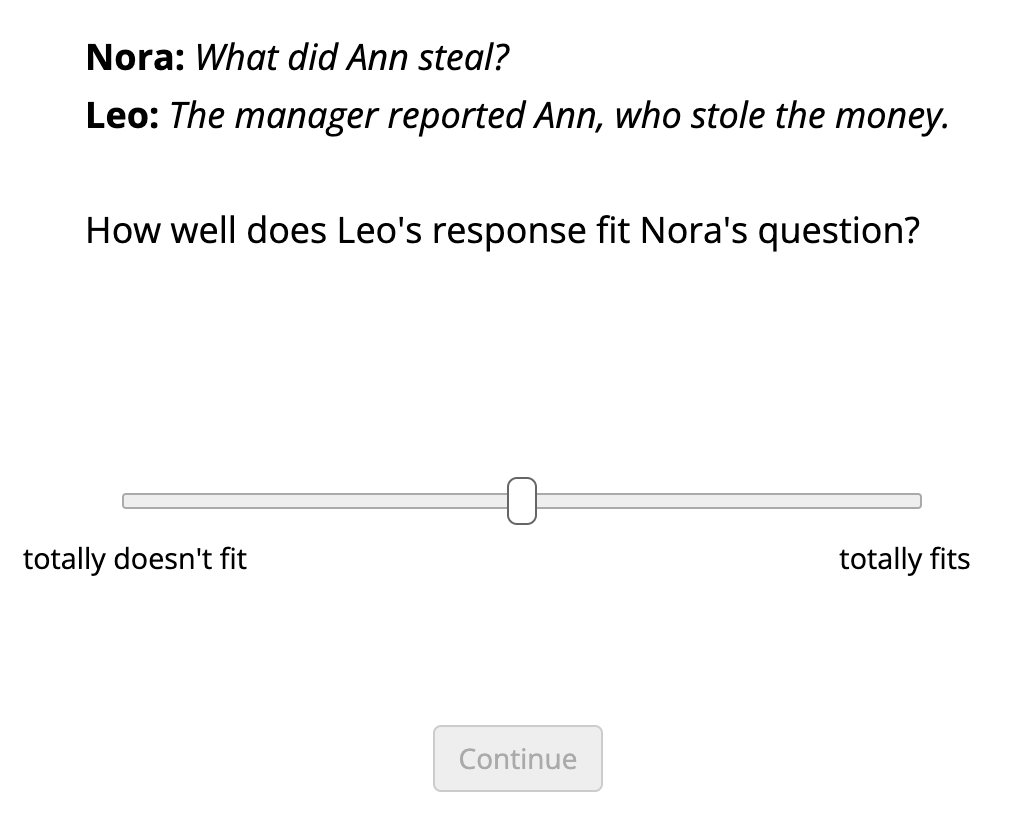
\includegraphics[width=\linewidth]{../../writing/paper/figures/trialExp1}}
					&
					\visible<2->{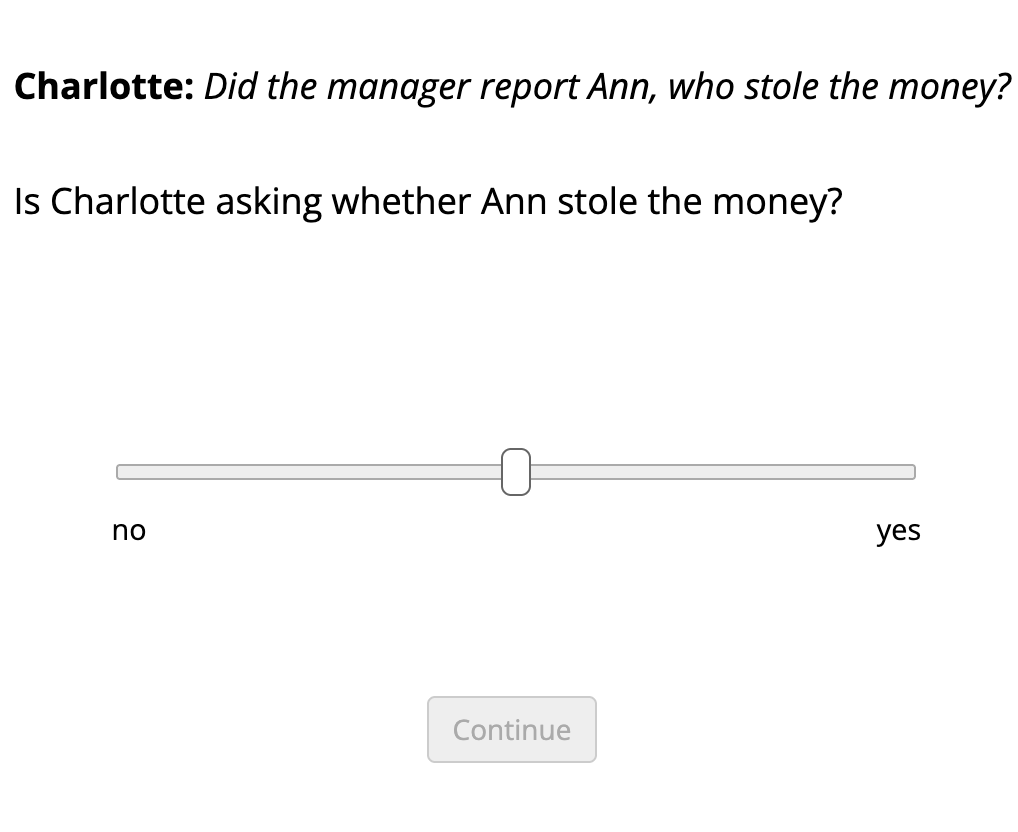
\includegraphics[width=\linewidth]{../../writing/paper/figures/trialExp2}}
					\\
					%
					{\visible<3->{\centering Exp.~3 (`direct dissent' diagnostic)}} &
					{\visible<4->{\centering Exp.~4 (`yes, but' diagnostic)}} \\
					%
					\visible<3->{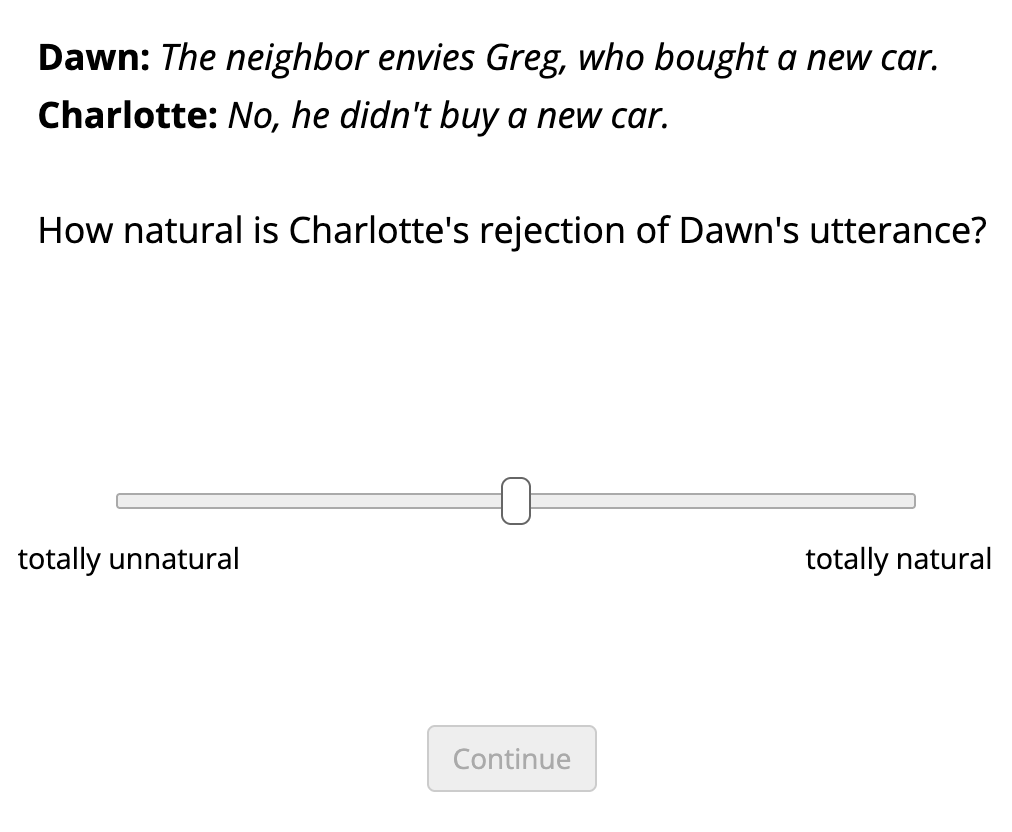
\includegraphics[width=\linewidth]{../../writing/paper/figures/trialExp3}}
					&
					\visible<4->{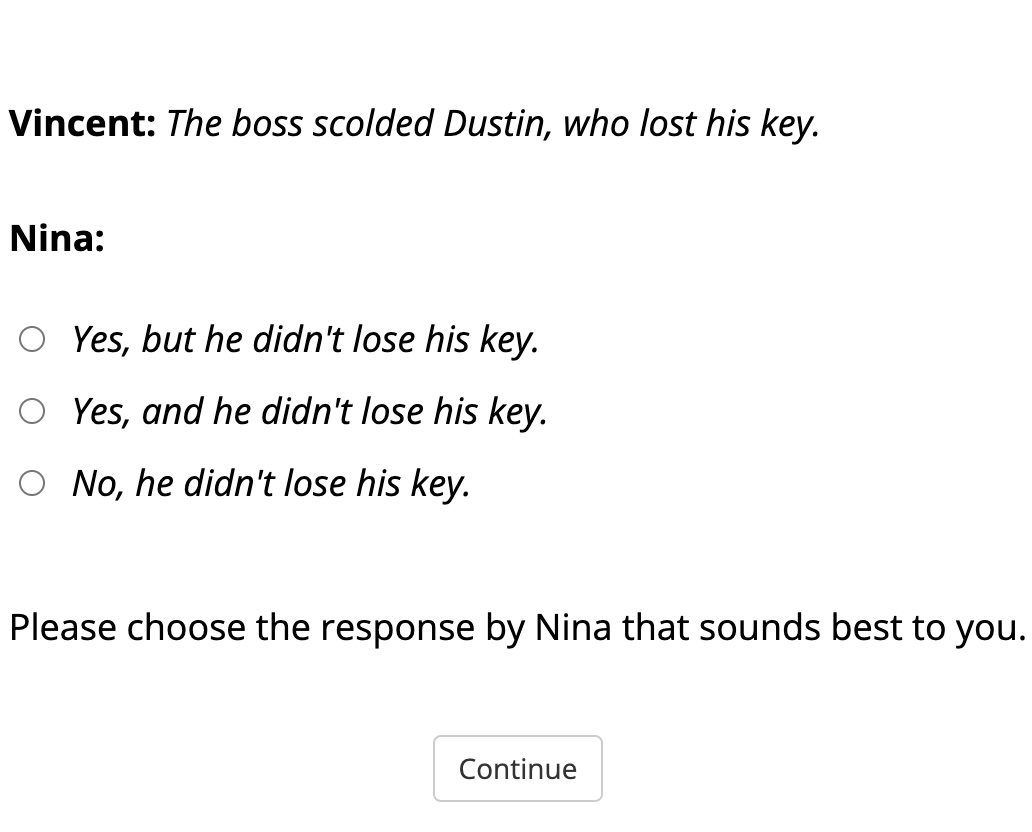
\includegraphics[width=\linewidth]{../../writing/paper/figures/trialExp4}}
					\\
				\end{tabular}
			\end{center}
			
	\end{frame}

	% \begin{frame}[t]\frametitle{Differences}\scriptsize
	
	% 	\begin{itemize}
	% 		\item Question-based vs. assertion-based diagnostics: Assumptions are different (\citealt{snider_anaphoric_2017,snider_at-issuenessne_2017,snider_distinguishing_2018,koev_notions_2018,faller_discourse_2019,korotkova_evidential_2020})
	% 		\item Medial appositive RCs usually not-at-issue on all four diagnostics (\citealt{potts_logic_2005,amaral_review_2007,tonhauser_diagnosing_2012,syrett_experimental_2015,destruel_cross-linguistic_2015,tonhauser_how_2018,solstad_cataphoric_2024})

	% 		\item BUT final appositive RCs have been argued that sentence-final appositive NRRCs can be interpreted as at-issue, based on findings from the direct-dissent diagnostic (\citealt{syrett_experimental_2015,anderbois_at-issue_2015})

			
	% 		\item Fine-grained lexical differences for the at-issueness of the embedded content of clause-embedding predicates \citealt{tonhauser_how_2018,degen-tonhauser-glossa}: e.g., $A$ \emph{knows} $p$ and $A$ \emph{is right} that $p$ are usually thought to come with inference that $p$ is true, but they differ in at-issueness ratings for propositional content $p$

	% 		% 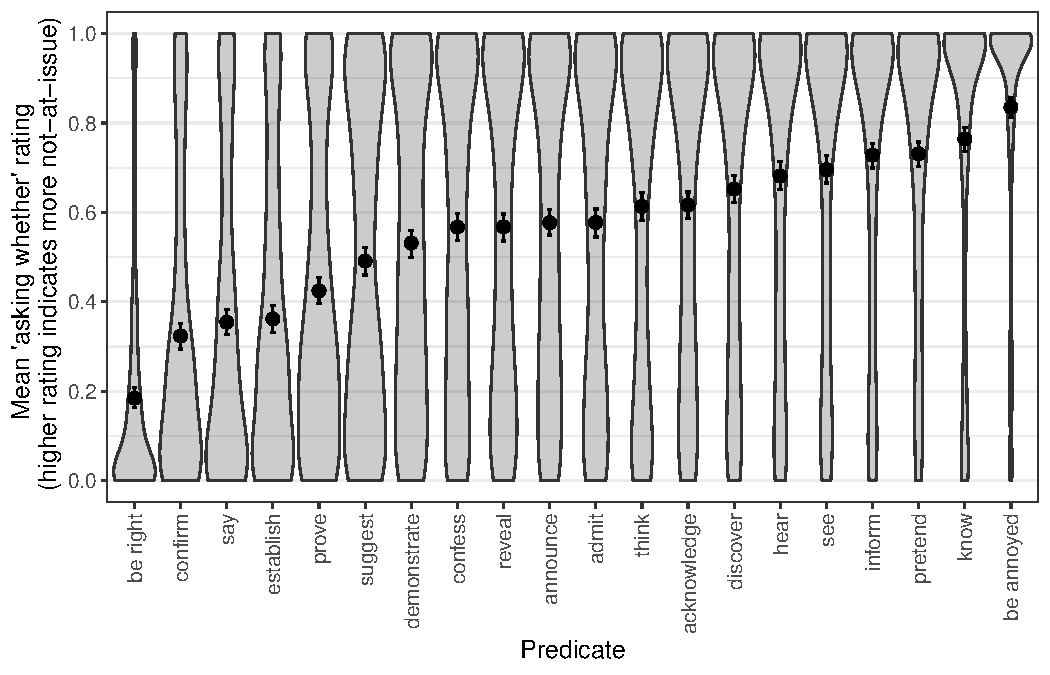
\includegraphics[width=0.5\textwidth]{../../results/degen-tonhauser-glossa/graphs/mean-asking-whether-ratings.pdf}

	% 		\item Can we find these differences?
	% 	\end{itemize}
	
	% \end{frame}


\section{Experiments 1–4: Results}

	\begin{frame}[t]\frametitle{Results}\scriptsize
		\vspace{-2\baselineskip}
			\begin{center}
			\begin{tabular}{p{.4\linewidth} p{.4\linewidth}}
				{\centering Exp.~1 (QUD diagnostic)} &
				{\centering Exp.~2 (`asking whether' diagnostic)} \\
	      		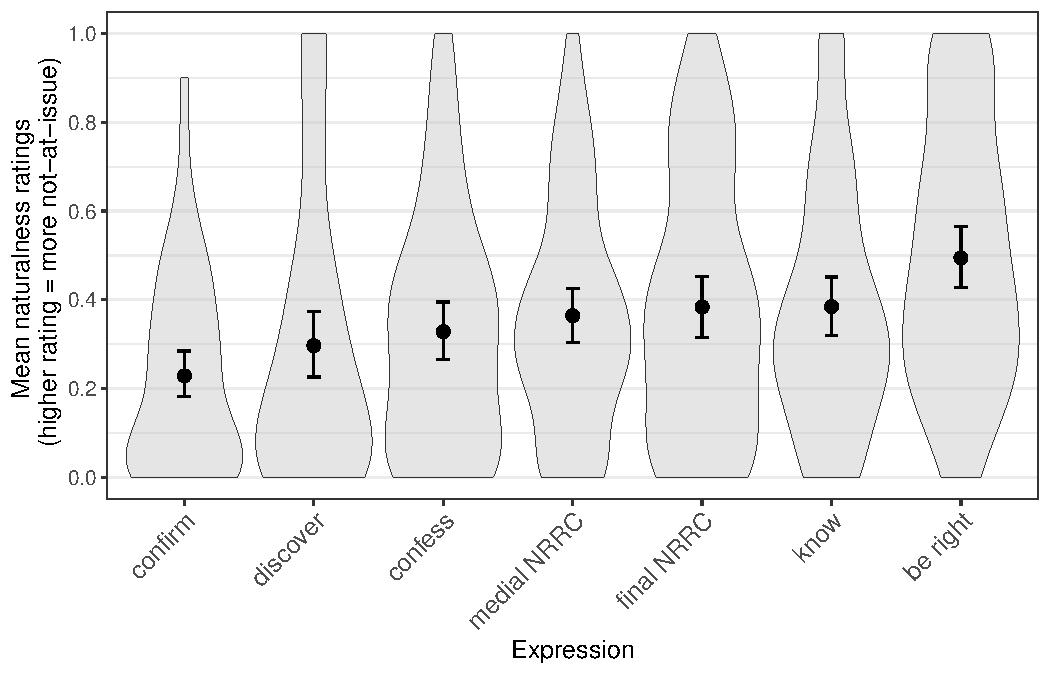
\includegraphics[width=\linewidth]{../../results/exp1/graphs/mean-ratings.pdf}
	      		&
	      		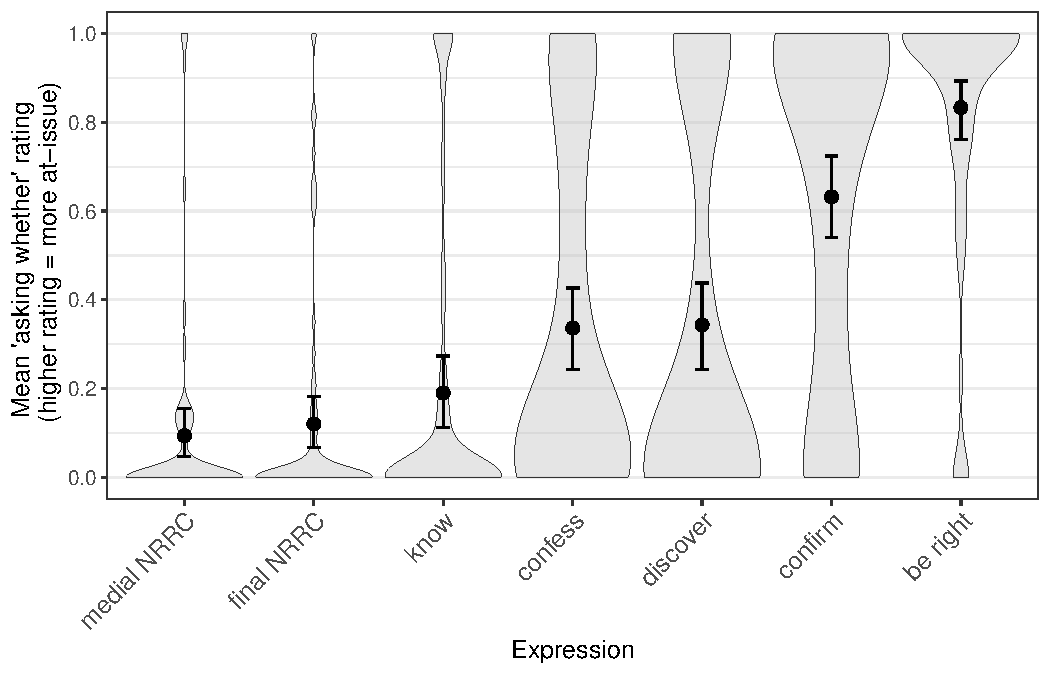
\includegraphics[width=\linewidth]{../../results/exp2/graphs/mean-ratings.pdf}
	      		\\
	      		{\centering Exp.~3 (`direct dissent' diagnostic)} &
				{\centering Exp.~4 (`yes, but' diagnostic)} \\
	      		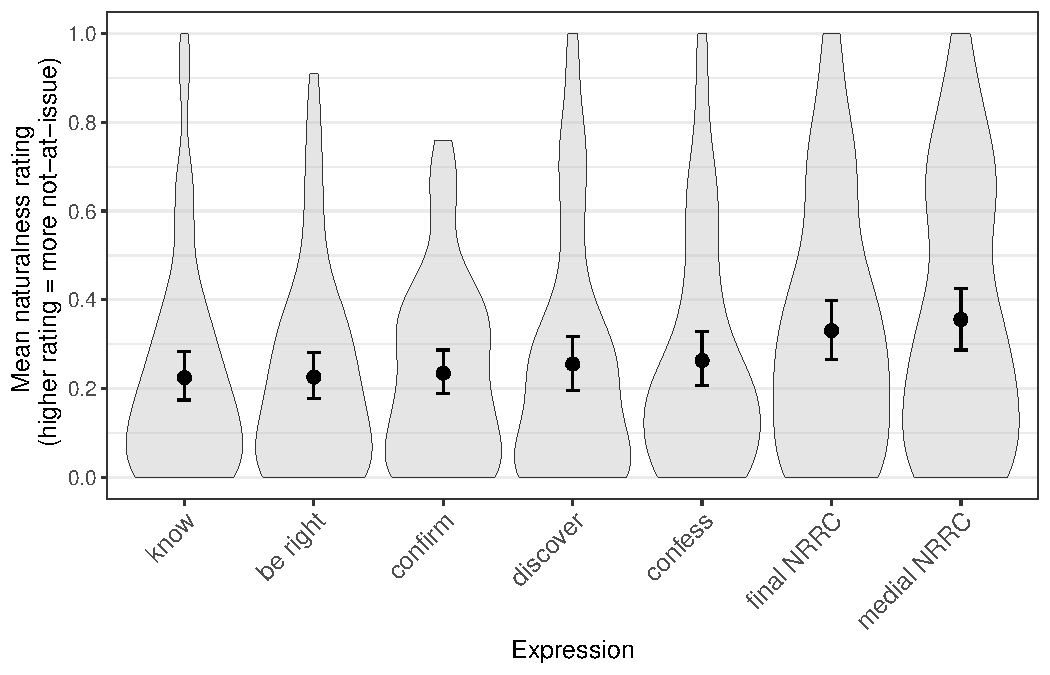
\includegraphics[width=\linewidth]{../../results/exp3/graphs/mean-ratings.pdf}
	      		&
	      		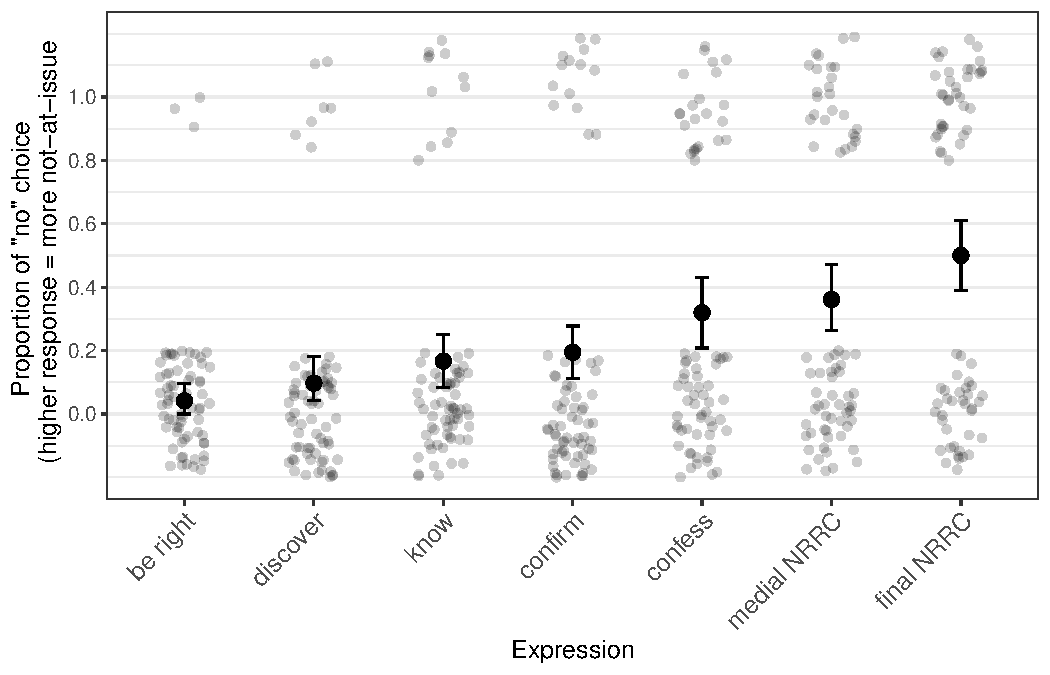
\includegraphics[width=\linewidth]{../../results/exp4/graphs/mean-ratings.pdf}
	      		\\
			\end{tabular}
		\end{center}
	
	\end{frame}

	\begin{frame}[t]\frametitle{Some observations}\scriptsize
		\begin{itemize}
			\item Experiment 2 (asking whether) shows the greatest differentiation between the contents, Experiment 2 (`direct dissent') showing the least; (range of means, and significant differences between them)

			\item rankings are very different (confirm always lower than discover)
			\item start w exp 2 / overlay w other diagrams that show statistical analysis

			\item No difference between medial and final NRRCs

			\item  (posthoc pairwise comparisons of the estimated means/proportions for each content using the `emmeans' package (\citealt{emmeans}) in R (\citealt{r}). The input to the pairwise comparisons were mixed-effects beta regression models (Exps.~1-3) or a mixed-effects logistic regression model (Exp.~4))

		\end{itemize}
	
		% Spearman rank correlations between the results of Exps.~1-4.:
		% \begin{center}
		% 	\begin{tabular}{l | c c c c}
		%     & Exp.~1 & Exp.~2 & Exp.~3 & Exp.~4 \\ \hline
		%     Exp.~1 (QUD diagnostic) & \cellcolor{lightgray} & .11 & -.29 & -.18 \\
		%     Exp.~2 (`asking whether' diagnostic) & \cellcolor{lightgray} & \cellcolor{lightgray} & .64 &.79 \\
		%     Exp.~3 (`direct dissent' diagnostic) & \cellcolor{lightgray}& \cellcolor{lightgray} & \cellcolor{lightgray} & .79  \\
		%     \hline
		%     % Exp.~4 (`yes, but' diagnostic) & & & & \cellcolor{lightgray} \\ \hline
		%     \end{tabular}
		% \end{center}
		
		%   \begin{itemize}
		%   	\item High correlation of 2 and 3 with 4 $.79$, and between 2 and 3 $.64$, but Exp.~1 shows low correlation with the rest
		%   \end{itemize}
	
	\end{frame}

	\begin{frame}[t]\frametitle{Some points}
		\begin{itemize}
			\item We do see differences between diagnostics, importantly not all show the same differences between contents 
			\item none of our diagnostics replicate the finding from S+K that final appositives are more at issue than medial ones
			\item only one replciate degen + tonhauser
		\end{itemize}	

		We could make some points here
		\begin{enumerate}
			% \item Why Exp.~1 is so different from the others (\emph{be right})
			% \item 
			\item And why Exp.~2 shows a greater differentiation than the others
		\end{enumerate}
		
		We focus on point 3 here
	
	\end{frame}

\section{Experiments 5--6}
	\begin{frame}[t]\frametitle{Two hypotheses}
		why is asking whether so different
		\begin{itemize}
			\item q-at-issuenes (thats not it)
			\item question embedding  (hypotheses)
			\item response task
			
		\end{itemize}
	
	\end{frame}

	\begin{frame}[t]\frametitle{Materials + procedure}
	
		screenshots
	
	\end{frame}

	\begin{frame}[t]\frametitle{Q-at-issueness or question-embedding?}\scriptsize
		
		Why is `asking whether' different from all others, when the QUD-one should be like the `asking whether' test based on Q-AI-ness?

		In experiments 5 and 6, we test whether the fine-grained differences among clause-embedding predicates observed with one diagnostic (asking-whether) are replicated with other diagnostics.
		  % \begin{itemize}
		  %   \item CCs of clause-embedding predicates because one diagnostic found fine-grained differences
		  %   \item Are these differences between contents replicated by the use of other diagnostics?
		  % \end{itemize}

		\ex.
	    \a.\label{exp5} Exp.~5 (`asking whether' diagnostic )
	    \\ {\bf Nora:} \emph{Is xx right that Lucy broke the plate?}
	    \\ Question to participants: Is Nora asking whether Lucy broke the plate?
	    \b.\label{exp6} Exp.~6 (`direct dissent' diagnostic)
	    \\ {\bf Nora:} \emph{Is XX right that Lucy broke the plate?}
	    \\ {\bf Leo:} \emph{Yes, she didn't break the plate.}
	    \\ Question to participants: How natural is Leo's response to Nora's question?
	
	\end{frame}

	\begin{frame}[t]\frametitle{Results}\scriptsize

	      \centering
	      \begin{tabular}{p{.48\linewidth} p{.48\linewidth}}
	      	Exp.~5 (`asking whether' diagnostic)
	      	&
	      	Exp.~6 (`direct assent' diagnostic)\\ 
	      	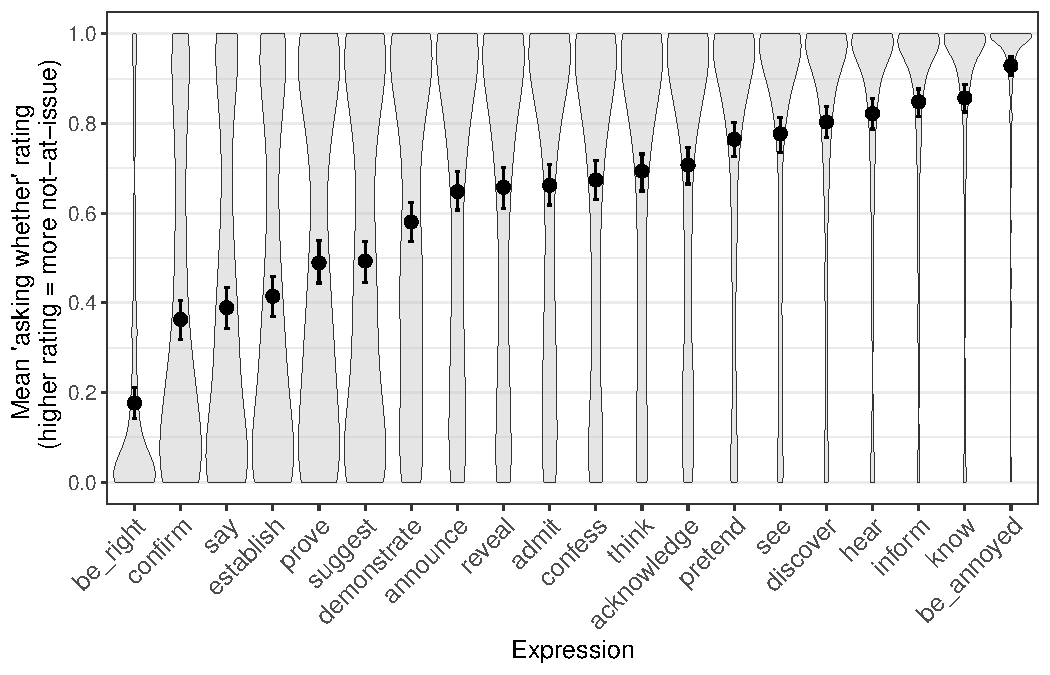
\includegraphics[width=\linewidth]{../../results/exp5/graphs/mean-ratings.pdf}%
	      	&
	      	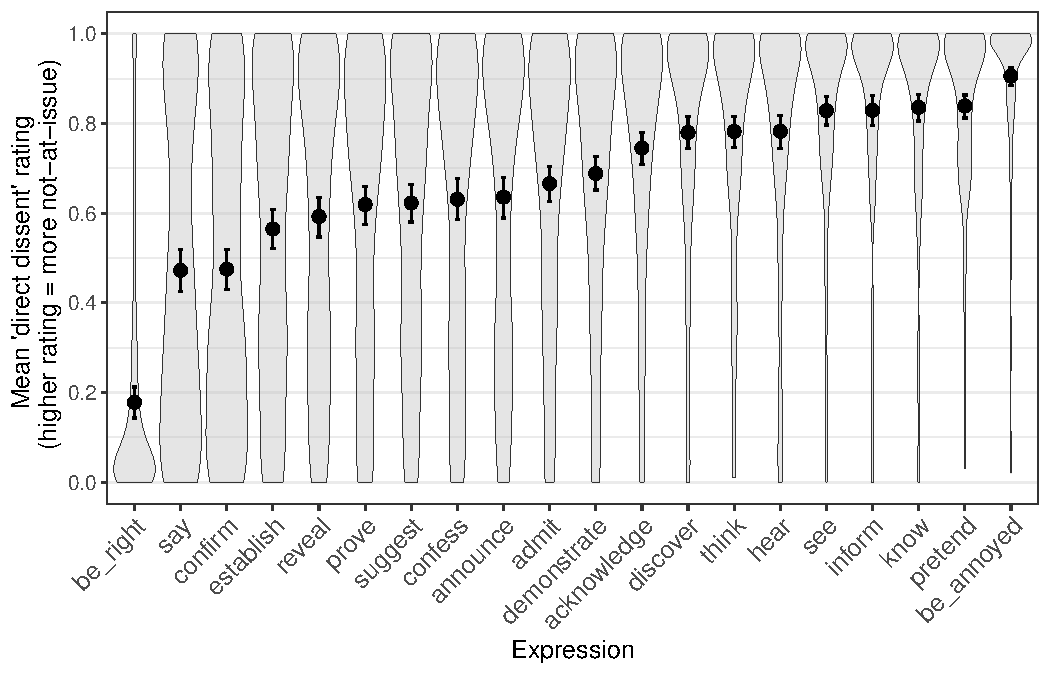
\includegraphics[width=\linewidth]{../../results/exp6/graphs/mean-ratings.pdf}
	      	\\
	      \end{tabular}

	      Results of Exps.~5-6. The panels show the mean ratings by expression for (a) Exp.~5 (asking whether diagnostic) and (b) Exp.~2 (direct assent diagnostic). Error bars indicate 95\% bootstrapped confidence intervals. Violin plots show the kernel probability density of individual participants' ratings.

	      \begin{itemize}
	      	\item Spearman rank = .93
	      \end{itemize}
	
	\end{frame}

	\begin{frame}[t]\frametitle{Discussion}
		
		\begin{itemize}
			\item These two are highly correlated 
			\item Answer to quesiton. not about response task, but interrogative embedding
			\item in relation to previous literature which is about q-at-issueness

			
		\end{itemize}

	\end{frame}	

\section{General discussion}
	
	\begin{frame}[t]\frametitle{Takeaways}
	
		\begin{itemize}
			\item it matters which diagnostic you use (experimental confirmation for snider, korotkova)
			\item difference between Q-at-issuenes doesnt seem to be the most important difference, but more where is the content embedded 
			\item no replication of Syrett + koev
			\item What the results might tell us about whether the diagnostics diagnose a shared underlying property
			\item Interaction of lexical semantics and pragmatics: Q
		\end{itemize}
	
	\end{frame}

	\begin{frame}[t]\frametitle{Interrogatives}
	
		why are interrogatives like that?

		\begin{itemize}
			\item 
		\end{itemize}
	
	\end{frame}

\begin{frame}[allowframebreaks]{\bfseries\opt References}
	\footnotesize
	\bibliographystyle{../cslipubs-natbib}
	\bibliography{../at-issueness}

\end{frame}

\end{document}